\graphicspath{ {imgs/} }
\documentclass[main.tex]{subfiles}
\begin{document}
\chapter{Bandit A/B Testing}
\section{Underlying Idea}
The previous chapter dealt with optimization concerning classical A/B Testing. The following will describe a fundamentally different approach in which there is no separation between the exploration and the exploitation phase. This is motivated by the idea that valuable costumers could be lost during exploration. Basically this means that we want to already maximize our profit while gaining information about the other buckets. When combining exploration and exploitation one has to choose on each step if a known good bucket should be used again or if one invests in other unknown buckets to gain more information about their reward function. This balancing is at the core of the now described algorithms.

\subsection{Bandit Algorithms}
Bandit algorithms originate from Machine Learning where they serve learning agents to show sensible behavior while exploring the environment. In each time step an agent is forced to make a choice among several actions. An action will lead to a reward. The reward function for any action is not known from the beginning and the agent can only estimate the true reward function of any action by trying this action. The objective is of course to maximize the received reward over the whole experiment. The name of this class of algorithms stems from their relation to the famous casino slot machines. Each action can be imagined as one lever in a row of many one-armed bandits. Each machine has a hidden reward function and a player wants to maximize their earned money at the end of the evening. The update rule for each step can be roughly formalized as:
\begin{align*}
NewEstimate \leftarrow OldEstimate + StepSize[Target - OldEstimate]
\end{align*}
A K-armed bandit problem is defined by random variables $X_{i,n}$ for $1 \leq i \leq K$ and $n\geq1$ where each $i$ is the index of a slot machine. Successive plays of machine i yield reward $X_{i,1},X_{i,2},...$ which are independent and identically distributed according to an unknown law with unknown expectation $\mu_i$. The machines are also independent.

\subsection{Reformulating A/B Testing}
Each new user is our chance to either explore or exploit what we know about the buckets of the test. Each assignment becomes the pull on a lever. Since we only measure each user once, the assignments are independent and identically distributed. We deal with a stationary environment which means our $StepSize$ is $\frac{1}{k}$ where $k$ denotes the number of assignments. Since we use no prior knowledge there is also no \emph{side information}. The reward value does not differ among the different levers. It is always $1$, although it could be in fact another fixed value. Later on described algorithms do sometimes require the reward of a lever to be bounded by a certain interval. For the sake of A/B Testing the concrete value should not matter and can be adapted as seen fit- it only has to be the same for each bucket. What does differ though is the real distributions underlying the variations we made in the buckets. Assume this distributions to be of the form $P_B(y|w)$ where $w$ are the unknown parameters that describe the distribution. By assigning users we generate random observations $D_B=(y_1,y_2..y_t)$. These observations are used to estimate the difference between the buckets. The experiment ends after a given number of trials - this number is called \emph{horizon}.

\section{Bandit algorithms}
\subsection{epsilon-greedy}
One of the simplest algorithms exploits always the best performing bucket (with the highest conversion rate) except for $\epsilon $'s fraction of cases where the next bucket is chosen uniformly. For example: if $\epsilon = 0.1$ every tenth assignment would not necessarily be to the best performing bucket. This also means that even after convergence for the bucket probabilities $10\%$ of the assignments would not always hit the optimal bucket. For $n$ buckets this would be:
\begin{align*}
P(exploration) \cdot P(\neg best machine | exploration) = \epsilon \cdot \frac{n-1}{n}
\end{align*}
times a not optimal result. A simulation with $1000$ tests with a horizon of $1000$ and varying $\epsilon$ gives the following plot for this algorithm:
\begin{figure}[ht]
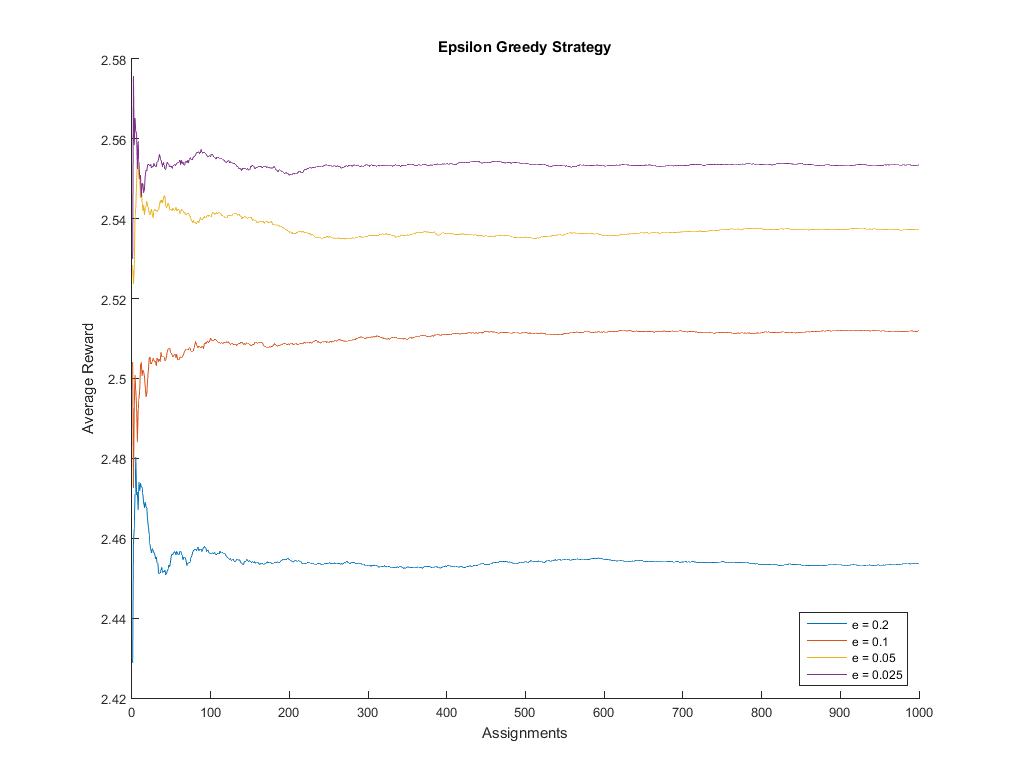
\includegraphics[scale=0.6]{epsGreedy.png}
\centering
\caption{Epsilon Greedy}
\label{fig:EpsGreedy}
\end{figure}
Note that this algorithm does not track or account for the uncertainty of the estimates it has about the buckets. And since it has no 'sense' for time (the Algorithm does not change if the experiment is nearly over and only $n$ choices left) the epsilon-greedy performs equally well if the environment changes and users behavior change later on.

\subsection{epsilon-first}
Another algorithm that is closely related is called the $\epsilon-first$ algorithm. This is close to A/B Testing since the exploration phase proceeds the exploitation phase for a finite number of steps and afterwards just exploits. This mimics the case where the tested change with the highest payoff is implemented and from then on permanently presented to all customers.
\begin{figure}[ht]
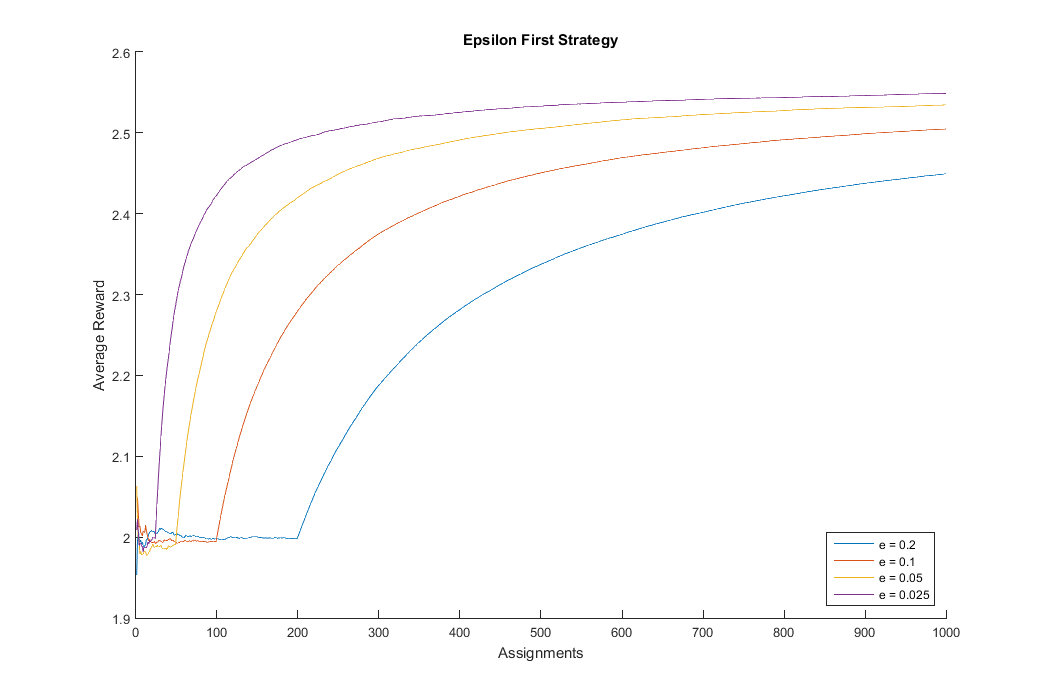
\includegraphics[scale=0.6]{epsFirst.png}
\centering
\caption{Epsilon First}
\label{fig:EpsiFir}
\end{figure}
Since the implementation is fixed after $\epsilon$ steps this algorithm can not react to changes that later on happen to the environment.

\subsection{Unified Confidence Bound}
The concrete formulas in this section are taken from ``Finite-time analysis of the multiarmed bandit problem'' by Auer~et~al.\,\cite{auer2002finite}, but the algorithm itself is known across the community. UCB (which stands for \emph{Uniform Confidence Bound}) does not explore for a fixed number of assignments, but dynamically changes the chances for not so good performing buckets to be chosen. The Hoeffding's inequality gives a confidence bound that models how sure we are about the estimated payoff across multiple plays. This way - the longer we do not play a machine the more likely it will be played in the future (but only once). We choose to play the next machine that maximizes:
\begin{align*}
mean(b_n) + \sqrt{\frac{2\log{N}}{n_p(b_n)}}
\end{align*}
Here $b_n$ is one of $n$ buckets and $n_p(b_n)$ is the number of times this bucket has been played. $N$ corresponds to the number of assignments across all buckets. This algorithm requires $mean(b_n)$ to be bounded by 1 so that the confidence bound overpowers the first term. This is given by our assumption that the concrete value of the individual rewards does not matter as long as they are the same across buckets. The fraction of time that is spend on exploring decreases exponentially.


\subsection{Thompson sampling}
This fairly simple algorithm was originally developed by William R. Thompson in his paper ``On the likelihood that one unknown probability exceeds another in view of the evidence of two samples''~\cite{thompson1933likelihood} To determine the next bucket to be played, the buckets probability distribution itself is used. The result of that sampling is used to update the buckets underlying distribution as described in the previous chapter.

\begin{algorithm}
\SetKwData{nb}{nextBucket}\SetKwData{nbs}{nextBucketSuccess}\SetKwData{i}{i}\SetKwData{r}{rew}
\SetKwData{nbf}{nextBucketFailures}
\SetKwArray{b}{buckets}\SetKwArray{d}{draws}
\SetKwFunction{max}{maxarg}\SetKwFunction{draw}{draw}\SetKwFunction{rw}{reward}
\KwIn{\b}
%\KwOut{\na}
\BlankLine
\d $\leftarrow$ zeroes \;
\ForEach{\i in \b }
{
\d(\i) $\leftarrow$ \draw{\b{\i}}
}
\nb $\leftarrow$ \max{\d} \;
\r = \rw{\nb}\;
\eIf{\r == 1}{
\nbs $\leftarrow$ \nbs + 1\;
}{
\nbf $\leftarrow$ \nbf + 1\;
}

\caption[Thompson Sampling]{The usage of Thompson sampling}
\label{alg:ThompsonSampling}
\end{algorithm}

They generate numbers that naturally balance between exploitation and exploration, because less performing buckets are demoted and winners promoted by the information already collected. This method is as well resistant to changes in the environment since they `notice' the change by playing a less performing bucket, that will then be played more often if its performance increased. A comparison between Thompson Sampling and the above described UCB-Algortihm can be found in \ref{fig:ThompsonVsUCB}. Here the UCB is weaker in the first part of Assignments but slightly outperforms the Thompson Sampling in the long run. A paper that is taking a look at the general performance of Thompson sampling versus UCB for more arms is ``An empirical evaluation of thompson sampling'' by Chapelle and Li \cite{chapelle2011empirical}. They show that in the general case Thompson sampling outperforms UCB.

\begin{figure}[ht]
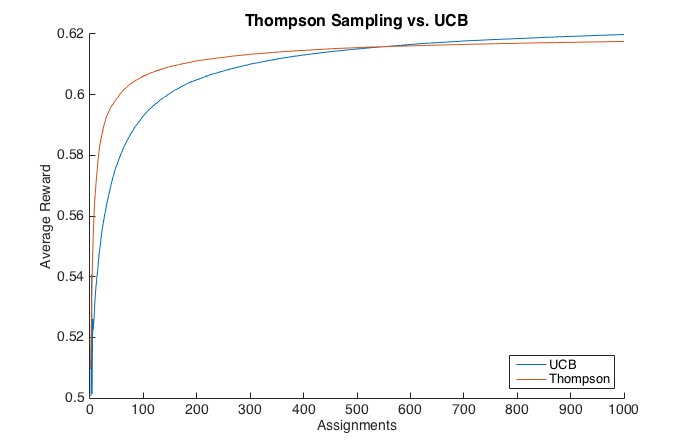
\includegraphics[scale=0.6]{ThompsonVsUCB.png}
\centering
\caption{Comparison for Thompson and UCB}
The graph averages $1000$ runs with random bucket distributions and a horizon of 1000.
\label{fig:ThompsonVsUCB}
\end{figure}

\subsection{Discussion}
The section started with a very weak Bandit algorithm: epsilon-greedy. The major drawback on that was the fact that the exploration phase did not adapt to the gained insights of the different buckets. But still: for this simplified scenario it works well compared to the other algorithms. This is due to the fact that only two buckets are compared and that their rewards do not change throughout the experiment.

UCB and Thompson Sampling are stronger Algorithms in the way, that they account for changes in the users behavior and their exploration phase is dynamically bound to the information that are collected during the test.

Bandit algorithms can be very useful when they keep on running even after the experimental phase is over. In fact, since most of them distribute new users in a way that over the time most of them experience the `better' variant, they replace the deployment cycle for new features by rolling them out slowly to the customer base.

\end{document}